%!TEX root = ../../main.tex
\section{Design og Implementering af Hardware}
Systemet består af følgende hardware blokke:
\begin{itemize}
\item RSConverter
\item Ventil-/pumpestyring
\item Flowsensor
\item Jordfugtsensor
\item pH-probe
\item Power Supply Unit (PSU)
\item Shields til Raspberry og PSoC
\end{itemize}

\subsection{RSConverter}
\begin{figure}[H]
	\centering
	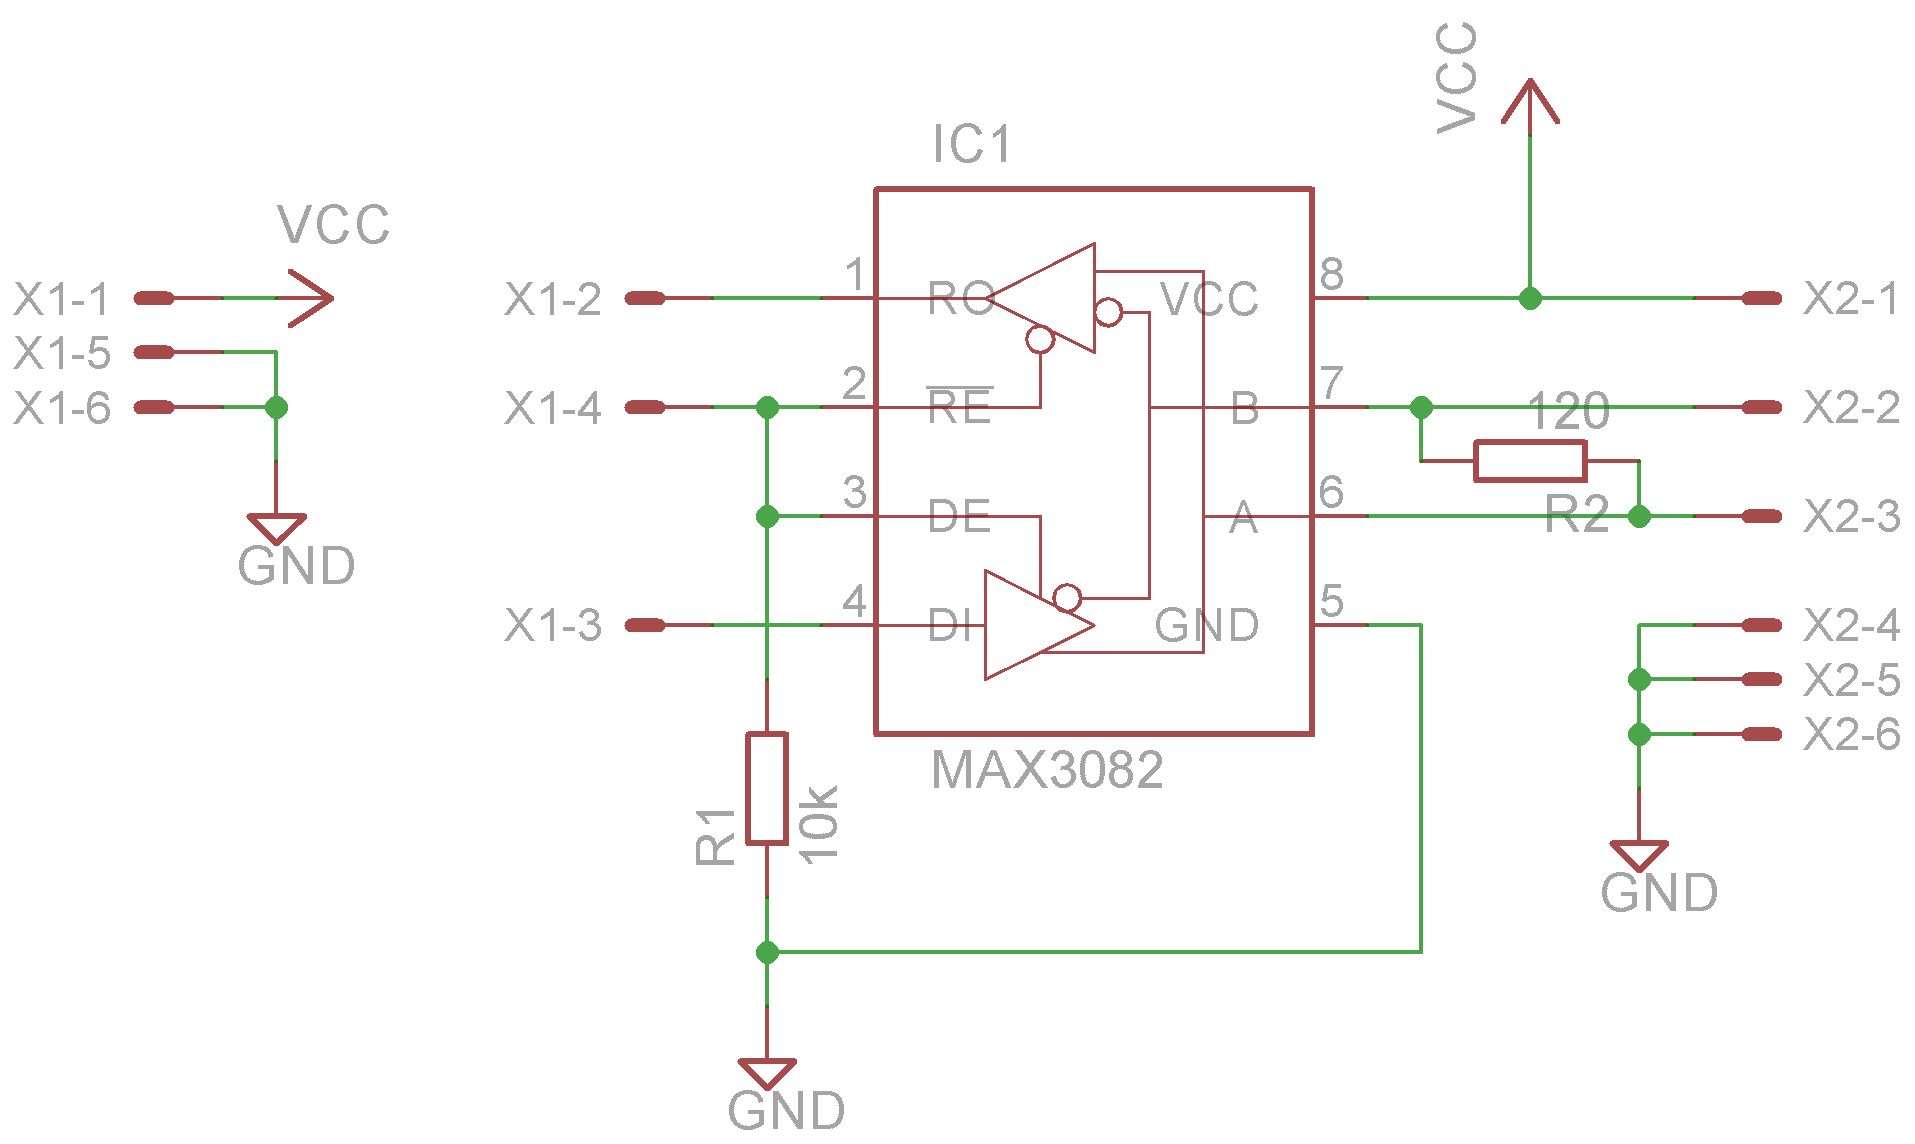
\includegraphics[scale=1]{Projektbeskrivelse/DesignOgImplementeringAfHW/RS485_Converter/Schematic}
	\caption{RS485 converter}
	\label{photo:RS485converter}
\end{figure}

Bussystemet som er valgt til at kommunikere på er RS485-standarden. Denne beskriver kun de hardwaremæssige krav og det er op til udvikleren selv at lave en protokol. RS485 udmærker sig ved at være en differentiel bus som giver mulighed for at kommunikere over længere afstande (op til 1200m). Der er forbundet arbejde med selv at udvikle en protokol, men det giver også mulighed for at skrue protokollen sådan, at den passer bedst til systemets behov.
\\\\
PSoC4 og Raspberry Pi understøtter dog ikke RS485-kommunikation. De kan begge kommunikere via. RS232/UART. Derfor er der udformet et simpelt RSConverter kredsløb som kan konvertere imellem RS232 og RS485. Kredsløbet benytter sig af MAX3082-kredsen. De eneste eksterne komponenter der er krævet er en pull-down modstand til at trække $TX_{enable}$ lav når den ikke er aktiveret fra PSoC4/Raspberry Pi. Til at terminere buslinjerne kræves en modstand som har samme modstand som det anvendte kabel. Dette gøres for at formindske reflektionen og dermed give det størst mulige signal i modtager-enden.

\subsection{Ventil-/pumpestyring}
Til at styring af ind- og afløbsventiler, samt vandpumpe benyttes en række MOSFET-styringskredsløb. MOSFET'erne er specifik valgt pga. af deres logic-level-kompatibilitet. Dette betyder at transistorens GATE kan kobles direkte til output-pin'en på PSoC'en, da dens grænseværdier følger CMOS-standarden. på fig.ref{screenshot:ventilStyringskreds}, s.\pageref{screenshot:ventilStyringskreds} ses eksempel på ventilstyringskreds.

\begin{figure}[H]
	\centering
	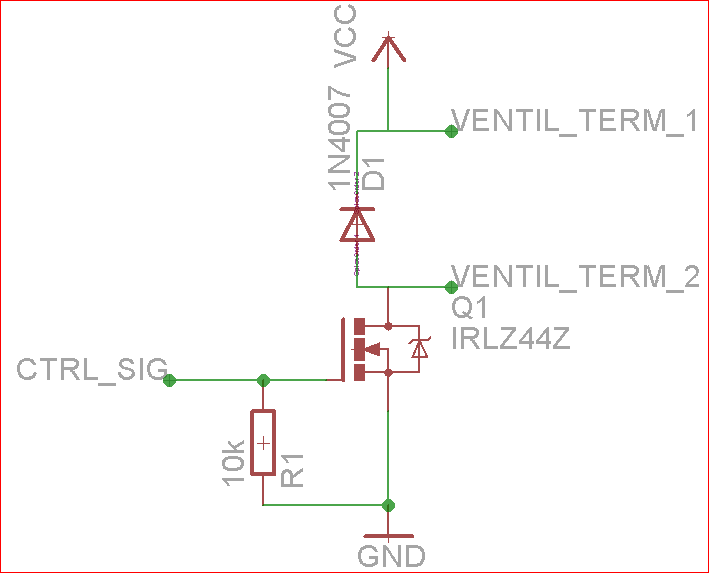
\includegraphics[scale=0.45]{Projektbeskrivelse/DesignOgImplementeringAfHW/Screenshots/VentilStyringskreds}
	\caption{Ventilstyringskredsløb}
	\label{screenshot:ventilStyringskreds}
\end{figure}

Både ventilerne, og pumpens belastning af styringskredsen har spolekarakter, da de indeholder et relæ som skal trækkes. Ved denne form for styring er det vigtigt at være opmærksom på, at når MOSFET'en går off, og spændingen fra spolen fjernes, hvorved strømmen ikke længere har en løbebane, vil spolen selv inducere en en modsatrettet spænding. Denne spænding kan blive utrolig høj, og i værste fald beskadige nærliggende komponenter så kredsløbet ikke længere er funktionelt.\newline 
Til at modvirke dette benyttes en flyback diode. Denne implementeres således at strømmen har en løbebane og herved kan spolen aflastes. Derudover benyttes der en pull-down modstand til at trække gat'en lav når den ikke er aktiveret af PSoC4'en.\\\


\subsection{Flowsensor}
Når karret skal fyldes med vand er det vigtigt at vide, hvor meget vand der i realiteten er fyldt i karret. Det blev derfor valgt at benytte en flowsensor til formålet. Jo mere vand som løber igennem sensoren jo højere en PWM-frekvens vil den sende ud på udgangen. Dette kræver dog, i praksis at der, over hele den tid hvor indløbsventilen er åben konstant skal holdes øje med det signal den leverer. Dette kræver alt opmærksomhed fra PSoC4'en, og i den konfiguration som vi benytter den, er dette ikke en mulighed.\newline
I stedet sætte karControl-programmet op til at modtage interrupts som triggeres af pulserne fra flowsensoren. Dette vil dog stadig kræve utrolig meget opmærksomhed fra karControl. For at imødekomme dennee problemstilling, er der udarbejdet et eksternt hardware counter-kredsløb. Dette kredsløb tæller pulserne fra flowsensoren, og når der er talt 10 pulser op, går en output-pin høj, og interrupt'et trækkes. Hermed minimeres antallet af interrupts og giver større frihed til karControl-programmet. På fig.\ref{screenshot:counter}, s.\pageref{screenshot:counter} ses schematics af det eksterne counter-kredsløb

\begin{figure}[H]
	\centering
	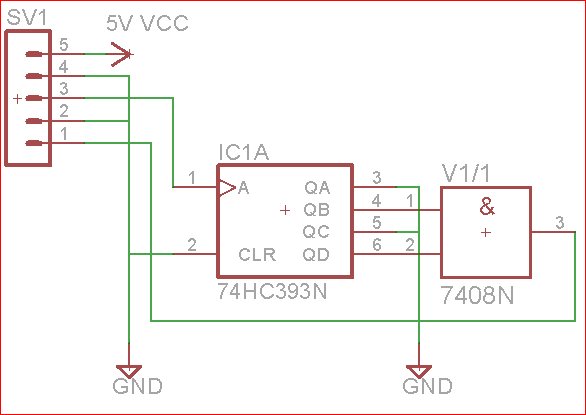
\includegraphics[scale=0.45]{Projektbeskrivelse/DesignOgImplementeringAfHW/Screenshots/FlowSensor_Schematics_ver1}
	\caption{Counter-kredsløb}
	\label{screenshot:counter}
\end{figure}

Kredsløbet er opbygget omkring en 4-bit counter (74HC393). Dertil er koblet en AND-gate som gør, at når counter'en rammer 10 giver den interrupt-signalet til PSoC4'en. Det allerførste der sker i ISR-rutinen er at tælleren nulstilles. Dette gøres for at undgå at der fejlagtigt gen-trigges når begge inputs til AND-gaten går høj 4 clockcycles senere når counter rammer 14 counts. 

\subsection{Jordfugtsensor}
Selve jordfugt sensoren skal måle jordfugten i jorden således systemet kan vide hvornår en plante skal have vand. 
Da vi ønsker at sensoren skal kommunikere over I2C igennem vores egen protokol, ønsker vi samtidig at levere en speciallavet jordfugt sensor med til systemet. Dette kræver at vi selv designer den. 
\\\\
Den første ide til at måle jordfugten gik ud på at måle den kapacitivt.  
Alt afhængig af jorfugtigheden må jordens ledeevne $\epsilon$r ændre sig. Dette kan måles ved hjælp af to elektriske ledende plader med jorden som dielektrikum. Der blev ud af noget printplade opbygget en pladekondensator. Til den hjemmebyggede pladekondensator blev der også opbygget en oscillator som varierede sin udgangsfrekvens afhængig af kondensatorens kapacitet. Dette kredsløb blev bygget med en LM555. Desværre var det umuligt af få oscillator-frekvensen til at være stabil og idéen blev derfor opgivet
\\\\
Anden idé var at lave en resistiv måling af jorden. Her stikkes et tobenet spyd ned i jorden og ved at sætte en spænding over det, vil strømmen ændres afhængig af fugtigheden. Dette viste sig også at være en dårlig metode, da der forekommer elektrolyse når der går en strøm i spyddet. For at undgå at slide mere end nødvendigt bruges der derfor en MOSFET til at lede strømmen i det øjeblik der måles.  
\\\\
Der blev tørret noget jord i en oven således fugtigheden var 0\%. Efterfølgende blev der tilsat vand i målte mænger, således der kunne tegnes en kurve over strøm afhængig af fugtighed. Ved hjælp af disse data kunne der laves en funktion i en mikroprocessor til at måle og udregne fugtigheden i procent. På figur \ref{photo:jordspyd_diagram} ses et diagram over jordspyddet. 

\begin{figure}[H]
	\centering 
	\includegraphics[scale=0.8]{Projektbeskrivelse/DesignOgImplementeringAfHW/Jordfugt_billeder/jordspyd.JPG}
	\caption{Diagram over jordspyddet}
	\label{photo:jordspyd_diagram}
\end{figure} 

Den valgte mikroprocessor blev en PSoC 4. I figur \ref{photo:PSoC_Creator} ses topdesignet over designet. 

\begin{figure}[H]
	\centering 
	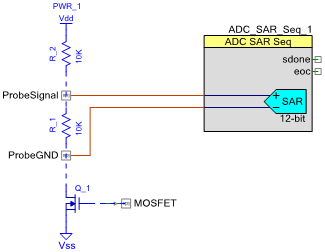
\includegraphics[scale=0.8]{Projektbeskrivelse/DesignOgImplementeringAfHW/Jordfugt_billeder/SAR_converter.png}
	\caption{Topdesign i PSoC creator}
	\label{photo:PSoC_Creator}
\end{figure} 

Da programmet var skrevet og testet blev der fremkaldt et print hvor selve mikroprocessoren skulle loddes på. Dette viste sig at volde nogle problemer da der ikke kunne komme nogen funktion ud af mikroprocessoren. Det var dog muligt at programmere den og det var derfor svært at finde ud af hvad der gik galt. I stedet blev der bygget et shield til PSoC 4 Pioneer kittet som blev brugt som prototype ved accepttesten. 

\subsection{pH-probe}
Planterne kræver ikke kun denne rette mændge vand, men også at vandet har den rette pH-værdi. pH-værdien i karret skal derfor måles samtidig med at der doseres gødning i karret. Til denne opgave blev valgt en glasprobe. Det viste sig at at være en meget godt metode at bruge da den både er billig og hurtig.
\\\\
Selve proben generere en spænding afhængig af pH-værdien. Det viste sig at proben har en udgangsimpedans på 9,5M\ohm og det tog noget tid at finde ud af hvorfor der ikke kunne måles noget med et oscilloskop. Problemet var at oscilloskopets indgangsimpedans var 1M\ohm og signalet blev derfor dæmpet betydeligt. For at løse problemet blev der koblet en buffer på udgangen af proben. Herefter var det hurtigt at omregne spændingen til pH-værdi i en PSoC 4. 
\\\\
Fordi at proben vil drifte med tiden kræver det at den kalibreres ca hver måned. Til dette laves der en kalibreringsfunktion på PSoc'en som indlæser værdierne når der trykkes på en knap. På figur \ref{photo:Schematic_ph} ses diagrammet.

\begin{figure}[H]
	\centering 
	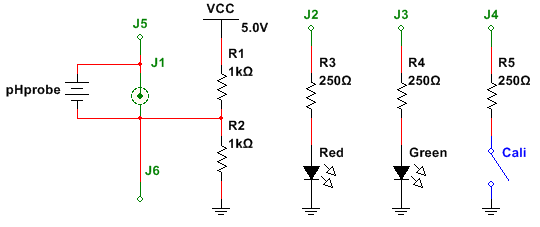
\includegraphics[scale=0.8]{Projektbeskrivelse/DesignOgImplementeringAfHW/pHbilleder/Schematic.png}
	\caption{Diagram over pH-proben}
	\label{photo:Schematic_ph}
\end{figure} 
På figur \ref{photo:PSoC_Creator_ph} ses topdesignet i PSoC creator.
\begin{figure}[H]
	\centering 
	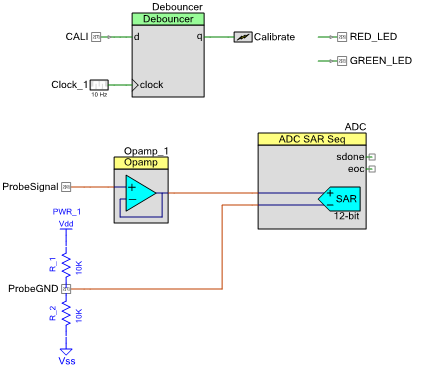
\includegraphics[scale=0.8]{Projektbeskrivelse/DesignOgImplementeringAfHW/pHbilleder/TopDesign.png}
	\caption{Topdesign i PSoC creator}
	\label{photo:PSoC_Creator_ph}
\end{figure} 
Der er foretaget en støjanalyse af proben ud fra den indhentede viden fra E/EP faget MSE (Mixed Signal Elektronik). Analysen viste at det største støjbidrag kom fra støjstrømmen i bufferen. Ved at lave en støjmåling af proben viste det sig at de forventede værdier var ca. en faktor 10 større. Ved høje impedanser blive strømstøjen meget dominerende. Det er derfor meget vigtigt at tage med i sin tanker/beregninger når det endelig kredsløb skal udformes.

\subsection{PSU}
For at forsyne systemet med de rigtige spændingerne og strømme er der udformet en strømforsyning. Den skal tilkobles 230VAC og forsyne systemet med 5V- og 12VDC. Dette kræver en transformering fra 230VAC til 12VAC og 2 reguleringskredsløb. Reguleringskredsløbet til 5V-forsyningen kan ses på figur~\ref{photo:PSU_5V}. Forskellen til 12V-forsyningen er $D_5$ og $R_4$.
 
\begin{figure}[H]
	\centering
	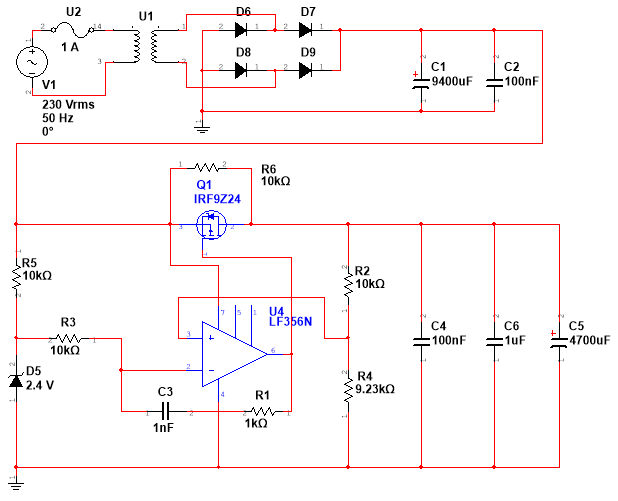
\includegraphics[scale=0.75]{Projektbeskrivelse/DesignOgImplementeringAfHW/PSU/PSU_5V}
	\caption{5V strømforsynings diagram}
	\label{photo:PSU_5V}
\end{figure}

Spændingen transformeres ned til 12VAC. Spændingen dobbeltensrettes og lades op på nogle store elektrolytter. $D_5$ skaber en reference spænding som fejlforstærkeren kan regulere ud fra. Spændingsdeleren $R_2$ og $R_4$ er udregnet således, at når spændingen på udgangen når over det ønskede punkt, vil fejlforstærkeren lukke for strømgennemløbet i MOSFET'en $Q_1$. For at undgå reguleringsstøj på udgangen er der koblet 2 kondensatorer og 1 elektrolyt på. Samtidig med er forstærkningen i fejlforstærkren gjort frekvens-afhængig hvilket ogsåundertrykker støjens indvirkning på reguleringen.
\\\\
Da der ved fuld belastning afsættes en forholdsvis stor effekt i de 2 regulerings-MOSFETs, er de placeret på en køleplade. 5V-forsyningen trækker en konstant strøm for at forsyne Raspberry Pi, PSoC4 mm. 12V-forsyningen belastes kun når der bruges pumper eller ventiler.

\subsection{Shields til Raspberry og PSoC}

Systemet består af mange små kredsløb, og mange af dem skal kobles til kar-PSoC'en. En almindelig løs kobling giver anledning til en del støj, og det er derfor er det valgt at placere alle disse kredsløb på såkaldte \emph{shields}. Der skal laves 3 forskellige:

\begin{itemize}
\item PiShield
\item Kar-shield
\item Ø-shield
\end{itemize}

Ved at samle kredsløbene på disse \emph{shields} opnår man langt færre "løse" ledninger imellem de forskellige blokke, da alle koblinger enten ligger i printlayout'et, eller er forbundet med pin-headers til kar-PSoC'en, som disse \emph{shields} passer sammen med. Dette reducerer samtidig med mulighed for støjindlejring fra omverdenen.
\\\\
At udlægge prints og teste disse er en forholdsvis stor opgave i forhold til at lave en prototype. Det giver dog et meget bedre overblik over systemet og reducerer muligheden for fejl. Der forekommer også leveringstid på udlagte print og det skaber et endnu større tidspres. Det er dog altid en god idé at designe print sideløbende med at kredsløbene tager form, så det er muligt i f.eks. næste iteration at skabe et fuldt funktionelt system som vil være tæt på det endelige.